% !TEX root = ../thesis.tex

\section{Numerical Methods}
\label{sec:numerics}

In this section the main numerical techniques implemented in \gls{hf} will be described. We will emphasize the critical role of the selected numerical discretization (\gls{fr} Method), and it capability to solve \gls{cfd} problems using unstructured meshes. 

\subsection{\gls{fr} Method}
\label{sec:frmethod}

What follows is an overview of the \gls{fr} framework. We start the discussion with the solution of the advection equation in one dimension using the \gls{fr} approach to illustrate the method and how it can be cast as a differential operator. Then we show how it would be possible to use \gls{fr} to discretize spatial derivatives of arbitrary order. We then proceed to describe which common schemes can be recovered via \gls{fr} and under which norm they can be proven to be stable. Then we explain how conservation equations can be solved in multiple dimensions. The \gls{ns} equations are a set of coupled conservation equations in multiple dimensions, so the extension of the \gls{fr} methodology to them uses the concepts explained here. The detailed description of the algorithm used in \gls{hf} is given by Castonguay et al. \cite{castonguay2011}.

\subsubsection{Solution of the General Advection Equation in One Dimension using the \gls{fr} Approach}

The \gls{fr} approach is a discretization of the $1^{\mathrm{st}}$ spatial derivative operator. The general advection equation is a good starting point to describe the mechanics of the scheme.

Consider the one-dimensional conservation law
\begin{equation}
\label{eq:cons_hf}
\frac{\partial u}{\partial t} + \frac{\partial f}{\partial x} = 0
\end{equation}

in domain $\Omega$, where $x$ is the spatial coordinate, $t$ is time, $u$ --the \emph{solution}-- is a scalar function of $x$ and $t$, and $f$ --the \emph{flux}-- is a scalar function of $u$. Note that by letting $f = f(u,\frac{\partial u}{\partial x})$, Equation~\ref{eq:cons_hf} becomes a model of the \gls{ns} equations.

Let us partition the domain $\Omega = [x_1,x_{N+1})$ into $N$ non-overlapping elements with 
interfaces at $x_1<x_2<...<x_{N+1}$. Then,
\begin{equation}
\Omega = \bigcup^N_{n=1} \Omega_n
\end{equation}
and $\Omega_n = [x_n,x_{n+1})$ for $n = 1,...,N$. To simplify the implementation, let us map each of the physical elements $\Omega_n$ to a standard element $\Omega_s=[-1,1)$ with the function $\Theta_n(\xi)$, where
\begin{equation}
x = \Theta_n(\xi) = \l( \frac{1-\xi}{2} \r) x_n + \l(\frac{1+\xi}{2}\r) x_{n+1} 
\end{equation}

With this mapping, the evolution of $u$ within each $\Omega_n$ can be determined with the following 
transformed conservation equation
\begin{equation}
\frac{\partial \hat{u}}{\partial t} + \frac{1}{J_n}\frac{\partial \hat{f}}{\partial \xi} = 0
\end{equation}
where
\begin{equation}
\hat{u} = u(\Theta_n(\xi),t) \text{ in } \Omega_n
\end{equation}
\begin{equation}
\hat{f} = f(\Theta_n(\xi),t) \text{ in } \Omega_n
\end{equation}
\begin{equation}
J_n = \frac{\partial x}{\partial \xi} \bigg|_{\Omega_n}
\end{equation}

Now, we introduce polynomials of degree $p$, $\hat{u}^\delta$ and $\hat{f}^\delta$, to approximate the exact values $\hat{u},\hat{f}$, respectively. We can write these polynomials as
\begin{equation}
\hat{u}^\delta = \sum_{i=1}^{N_s} \hat{u}_i^\delta l_i(\xi)
\end{equation}
\begin{equation}
\hat{f}^\delta = \sum_{i=1}^{N_s} \hat{f}_i^\delta l_i(\xi)
\end{equation}
where $N_s$ is the number of solution points, $\hat{u}_i^\delta$ is the current value of the 
solution approximation function at the $i^\text{th}$ \emph{solution point} in the reference element, 
$\hat{f}_i^\delta$ is the current value of the flux approximation function at the $i^\text{th}$ 
\emph{flux point} in the reference element, $l_i$ is the Lagrange polynomial equal to $1$ at the 
$i^\text{th}$ solution point and $0$ at the others, and $\delta$ denotes that the function is an 
approximation.

Note that the piecewise polynomials might not be continuous (or $C^0$) across the interfaces. In the 
\gls{fr} approach, the flux used in the time advancement of the solution is made $C^0$ 
by introducing flux correction functions.

This can be achieved by finding interface solution values at each element boundary and then correcting the 
solution. Let $\hat{f}_L^{\delta I}$ and $\hat{f}_R^{\delta I}$ be the interface solution values at left and right 
boundaries of some element, respectively. $\hat{f}_L^{\delta I}$ and $\hat{f}_R^{\delta I}$ can be found with a Riemann solver for \gls{dg} methods\cite{hesthaven2007nodal}. Then, select solution correction functions $g_L$ and 
$g_R$ such 
that
\begin{equation}\label{eq:condition}
g_L(-1) = 1 \;,\; g_L(1) = 0
\end{equation}
\begin{equation}
g_R(-1) = 0 \;,\; g_R(1) = 1
\end{equation}
and let
\begin{equation}
\hat{f}^C = \hat{f}^\delta + (\hat{f}^{\delta I}_L - \hat{f}^\delta_L) g_L + (\hat{f}^{\delta I}_R 
- \hat{f}^\delta_R) g_R
\end{equation}
where superscript $C$ denotes the function is corrected, and $\hat{f}^\delta_L$, $\hat{f}^\delta_R$ 
represent the solution approximation evaluated at the left and right boundaries.

As a result, the \gls{fr} spatial differential operator in element $n$ can be written as

\begin{equation}
\begin{aligned}
\dd{f(x)}{x}\bigg|_{\Omega_n} &\stackrel{FR}{=} \frac{1}{J_n}\ddxi{\hat{f}^C(\xi)}\\ &= \frac{1}{J_n}\l(\sum_{i=1}^{N_s} \hat{f}_i^\delta \ddxi{l_i(\xi)} + (\hat{f}^{\delta I}_L - \hat{f}^\delta_L) \ddxi{g_L(\xi)} + (\hat{f}^{\delta I}_R 
- \hat{f}^\delta_R) \ddxi{g_R(\xi)}\r)
\end{aligned}
\end{equation}

The actual values of the corrected quantity $\hat{f}^C$ are never used, only its first spatial derivative.

%Using the values of $\hat{u}^\delta_i$ and $\frac{\partial \hat{u}^C}{\partial \xi}|_{\xi_i}$ we then find 
%$$\hat{f}_i^\delta = \hat{f}\l(\hat{u}^\delta_i,\frac{1}{J_n}\frac{\partial \hat{u}^C}{\partial \xi}\bigg|_{\xi_i}\r) \;\; \text{in element } \Omega_n$$
%We can proceed in a similar fashion to correct the flux to obtain
%\begin{equation}
%\hat{f}^C = \hat{f}^\delta + (\hat{f}^{\delta I}_L - \hat{f}^\delta_L) h_L + (\hat{f}^{\delta I}_R 
%- \hat{f}^\delta_R) h_R
%\end{equation}
%where $h_R$ and $h_L$ are right and left flux correction functions satisfying the same boundary 
%conditions as $g_R$ and $g_L$, respectively, and $\hat{f}_L^{\delta I}$ and $\hat{f}_R^{\delta I}$ are the interface fluxes found via a Riemann solver. Note that if the flux corresponds to linear advection, correcting the solution and correcting the flux are equivalent steps.

The solution can then be advanced at each solution point $i$. In semi-discrete form, this is
\begin{equation}\label{eq:semidiscrete_hf}
\frac{d \hat{u}_i^\delta}{d t} = - \frac{1}{J_n}\frac{\partial \hat{f}^C}{\partial \xi}(\xi_i)
\end{equation}

\subsubsection{Extension to Higher Order Spatial Derivatives}

\gls{fr} can be used to discretize spatial differential operators of any order via composition. For example, the second derivative spatial differential in element $n$ can be discretized as

\begin{equation}
\begin{aligned}
\frac{\partial^2 *}{\partial x^2}\bigg|_{\Omega_n} &= \dd{}{x}\l(\dd{*}{x}\r)\bigg|_{\Omega_n}\\
& \stackrel{FR}{=} \frac{1}{J_n} \dd{}{\xi}\l( \frac{1}{J_n} \dd{*^C}{\xi}\r)^C
\end{aligned}
\end{equation}

Each differential operator requires the correction of the operand. Then, in the case of the second derivative operator, $*$ is corrected once using its values at each element boundary point, the common $*$ values at each boundary point, and its values at each internal point. This provides the values of $\dd{*^C}{\xi}$ at each internal point.

Let $q = \frac{1}{J_n} \dd{*^C}{\xi}$. We can find the values of $\dd{q^C}{\xi}$ using the same procedure we used to find $\dd{*^C}{\xi}$.

As a result, the \nth{m} \gls{fr} spatial derivative operator will require $m$ corrections.

\subsubsection{Energy Stability of \gls{fr} in the Linear Advection-Diffusion Equation}
The \gls{fr} scheme can be made provably stable for the linear advection-diffusion equation by selecting special types of correction functions~\cite{castonguay2013energy}. In general, these correction functions are polynomials of degree $p+1$ so both sides in Equation~\eqref{eq:semidiscrete_hf} are quantities related to polynomials of order $p$ --for consistency~\cite{huynh2007flux}.

Vincent et al.~\cite{vincent2011new} have shown that in the case of the 1-dimensional, linear advection equation, the \gls{fr} approach can be proven to be stable for a specific family of correction functions parameterized by a scalar called $c$. This parameter arises from the desire to ensure the following Sobolev-type norm is bounded above by zero

\begin{equation}
||u||^2_2=\sum_{n=1}^{N}\int_{x_n}^{x_{n+1}} \l\{ u^2 + 
\frac{c}{2} \l( \dd{^p \uud}{x^p} \r)^2 \r\} dx
\end{equation}

In the case of pure linear advection, they showed that by selecting specific values of $c$ it is possible to recover a particular nodal \gls{dg} and \gls{sd} methods plus a \gls{fr} scheme that was previously found to be stable by Huynh~\cite{huynh2007flux}. The family of schemes that are provably stable in the linear advection case are named \gls{esfr}. The coefficients that give rise to the correction functions that recover \gls{dg} and \gls{sd} schemes in the linear advection case are labeled $c_{DG}$ and $c_{SD}$, respectively. In addition, there is an \gls{esfr} scheme that maximizes the \gls{cfl} condition. This scheme's correction functions arise from selecting $c = c_{+}$.

Similarly, the families of schemes that are stable in the linear advection-diffusion equation have an additional parameter, which Castonguay et al. \cite{castonguay2013energy} labeled $\kappa$. The schemes arising from $\kappa_{DG}$ and $\kappa_{SD}$ recover the behavior of \gls{dg} and \gls{sd}, respectively, in the linear advection-diffusion equation. The scheme arising from $\kappa_{+}$ provides the largest \gls{cfl} condition.

It is important to keep in mind that the \gls{fr} schemes that recover other schemes in the linear equations can be used in non-linear equations, but the \gls{fr} schemes' non-linear properties will likely be different from those of the schemes they recover in the linear case. 
\subsubsection{Extension to Multiple Dimensions}
\label{sec:extension_multiple_dimensions}

Extension of \gls{fr} to multiple dimensions requires formulating multi-dimensional interpolation functions and correction functions that satisfy boundary conditions equivalent to those in Eqn.~\eqref{eq:condition} for each type of element.

Interpolation bases for quadrilaterals and hexahedra can be obtained via tensor products of the 1-dimensional interpolation basis. In \gls{hf}, the solution in hexahedra is discretized in the following way
\begin{equation}
{\hat{u}}^\delta(\xi,\eta,\zeta) = \sum_{i=1}^{p+1} \sum_{j=1}^{p+1} \sum_{k=1}^{p+1}
{\hat{u}}^\delta_{i,j,k} l_i(\xi) l_j(\eta) l_k(\zeta),
\end{equation}
where $i$, $j$, $k$ index the solution points along the $\xi, \eta, \zeta$ directions, respectively. The flux is discretized similarly.

The interpolation basis for triangles and tetrahedra are described in detail by Hesthaven and Warburton~\cite{hesthaven2007nodal}. Figure \ref{fig:tri_points} shows a possible configuration of internal and boundary points. The extension of interpolation polynomials to prisms is obtained via tensor products of the 1-dimensional basis with the triangular basis~\cite{castonguay2011}. 

The most general polynomial discretization of a $k$-dimensional solution scalar field and flux vector field in an arbitrary reference element is
\begin{align}
\label{eqn:general_u}
\hat{u}^\delta({\pmb \xi}) &= \sum_{i=1}^{N_s} \hat{u}_i^\delta {\phi}_i({\pmb \xi}),\\
\hat{\bf f}^\delta({\pmb \xi}) &= \sum_{i=1}^{N_s} \hat{\bf f}_i^\delta {\phi}_i({\pmb \xi}),
\end{align}
where $N_s$ is the number of solution points in an element, ${\phi}_i({\pmb \xi})$ is a polynomial basis function associated with solution point $i$ constructed such that ${\phi}_i({\pmb \xi}_j) = \delta_{ij}$ and $i,j = 1,\dots,N_s$.

By letting $\vec{u} = <\hat{u}_1^\delta, \hat{u}_2^\delta,\dots,\hat{u}_{N_s}^\delta>^T $, $\vec{\bf f} = <\hat{\bf f}_1^\delta, \hat{\bf f}_2^\delta,\dots,\hat{\bf f}_{N_s}^\delta>^T $, and $\vec{\phi} = <\phi_1,\phi_2,\dots,\phi_{N_s}>^T$ the discretization can be written more concisely as
\begin{equation}
\begin{split}
\hat{u}^\delta({\pmb \xi}) &= \vec{u}^T \cdot \vec{\phi}({\pmb \xi}) =  \vec{\phi}({\pmb \xi})^T\cdot \vec{u},\\
\hat{\bf f}^\delta({\pmb \xi}) &= \vec{\bf f}^T \cdot \vec{\phi}({\pmb \xi}) = \vec{\phi}({\pmb \xi})^T \cdot \vec{\bf f}.
\end{split}
\end{equation}

Note that we are using the boldface and arrow notation to denote vectors. Boldface vectors have a number of entries equal to the number of dimensions of the problem domain. Arrow vectors are vectors of general dimensions.

In the general \gls{fr} approach, the boundary conditions for the correction functions in multiple dimensions can be formulated as
\begin{equation}\label{eq:genConstraint}
{\bf{h}}_i( {\pmb \xi}_j)\cdot {\bf{n}}_j = \delta_{ij},
\end{equation}
where ${\bf{h}}_i$ is the correction vector function associated with interface point $i$, ${\pmb \xi}_j$ is the location vector of the $j^\text{th}$ interface point, and ${\bf{n}}_j$ is the outward unit normal at interface point $j$. Interface (or boundary) points are located on the boundary of an element.

One of the challenges in the \gls{fr} approach is finding correction functions that not only satisfy Equation~\eqref{eq:genConstraint} but also guarantee stability in the linear advection-diffusion case. Correction functions that guarantee such stability exist for 1-dimensional segments\cite{vincent2011new}, triangles\cite{castonguay2012new,williams2013tri}, and tetrahedra\cite{williams2013tet}. FR schemes with these correction functions comprise the ESFR family of schemes.

The update step at solution point $i$ and element $n$ in the \gls{fr} approach for the multidimensional advection equation $\frac{\partial u}{\partial t} + \nabla \cdot \vec{f} = 0$ becomes
\begin{equation}
\label{eqn:discrete}
\begin{split}
\frac{d {u}^\delta_i}{d t} &= - \frac{1}{\text{det}(\tilde{J_n})} \nabla \cdot {\bf f}_i^C({\pmb \xi}_i) = - \frac{1}{\text{det}(\tilde{J_n})} \nabla \cdot \l({\bf f}_i^\delta({\pmb \xi}_i) + \sum^{N_f}_{j = 1} \l[\l( \hat{\bf f}^{\delta I}_j - \hat{\bf f}^b_j \r)\cdot {\bf n}_j \r]\vec{\bf h}_j ({\pmb \xi}_i) \r)\\
&=- \frac{1}{\text{det}(\tilde{J_n})} \l( \nabla \cdot {\bf f}_i^\delta({\pmb \xi}_i) + \sum^{N_f}_{j = 1} \l[\l( \hat{\bf f}^{\delta I}_j - \hat{\bf f}^b_j\r)\cdot {\bf n}_j \r]\nabla \cdot\vec{\bf h}_j ({\pmb \xi}_i)\r)\\
&=- \frac{1}{\text{det}(\tilde{J_n})} \l( \vec{\nabla \phi}({\pmb \xi}_i)^T  \cdot  \vec{\bf f} + \sum^{N_f}_{j = 1} \l[\l( \hat{\bf f}^{\delta I}_j - \hat{\bf f}^b_j\r)\cdot {\bf n}_j \r]\nabla \cdot\vec{\bf h}_j ({\pmb \xi}_i)\r),\\
\end{split}
\end{equation}
where $N_f$ is the number of interface points, $\tilde{J_n}$ is the Jacobian matrix, $\vec{\nabla \phi}({\pmb \xi}_i)$ is the vector of gradients of each $\phi_i$ function evaluated at ${\pmb \xi}_i$, $\vec{\bf f}^\delta$ is a vector of flux vectors, and $\hat{\bf f}^b_j$ is the flux vector at the $j^{\text{th}}$ interface point (obtained via extrapolation).

Note that it is possible to evaluate each of the terms in Equation \eqref{eqn:discrete} for all $i = 1,\dots,N_s$ with a series of matrix-vector multiplications.

In terms of time integration, \gls{hf} uses an explicit Adaptive \gls{rk45} Method and local or global time stepping. Currently, a polynomial multigrid to improve the code convergence is being validated.

\subsection{Shock Capturing and Stabilization Models}

We use the method of concentration described in~\cite{Sheshadri2014} for detecting shocks on meshes with quadrilateral elements. We are still in the process of extending the method of concentration to triangles and are currently using Persson and Peraire's method~\cite{persson2006sub, Persson13} for the same. We have explored both selective addition of artificial viscosity as well as modal order reduction for capturing the detected shocks effectively. Persson and Peraire have used this shock capturing tool as a stabilization method as well in their turbulence calculations. Here we show a viscous case on quadrilateral elements using the concentration method (reproduction of the result in \cite{Sheshadri2014}) and an inviscid case on triangles using Persson and Peraire's method. \\

 Figures \ref{fig:visM1pt2-density} and \ref{fig:visM1pt2-energy} show the density and energy plots for a \gls{ma} 1.2 flow over a NACA 0012 airfoil at a 5$^{\circ}$ angle of attack. The flow is at \gls{re} of 60000 and we have used 6th order polynomial interpolation in the elements for the computation. There is a bow shock in front of the airfoil and we see fish-tail shocks at the trailing edge. We can also see boundary layer formation and a $\Lambda$-shock structure on the upper side of the airfoil. Here we have used simple modal order reduction in elements with shock sensor value above a threshold. Figure \ref{fig:sensor} shows the elemental shock sensor values. We can see the shock sensor is able to distinguish between shocks and other smooth regions enabling the structure of the vortices and boundary layer to be preserved. \\
 
 Figure \ref{fig:inv_mach} shows an inviscid flow of \gls{ma} = 1.6 over a NACA 0012 airfoil at $0^{\circ}$ angle of attack on a triangle mesh. Here we use Persson and Peraire's method  for shock detection and can see that we the shock has been detected and captured well. A few oscillations still remain near the strong bow shock in front of the airfoil even after enforcement of continuity of the artificial viscosity coefficients. Figures ~\ref{fig:AV-ele} and ~\ref{fig:AV-cont} show the artificial viscosity being added element-wise and after continuity enforcement respectively.

\begin{figure}
\centering
\begin{minipage}[t]{.5\textwidth}
  \centering
  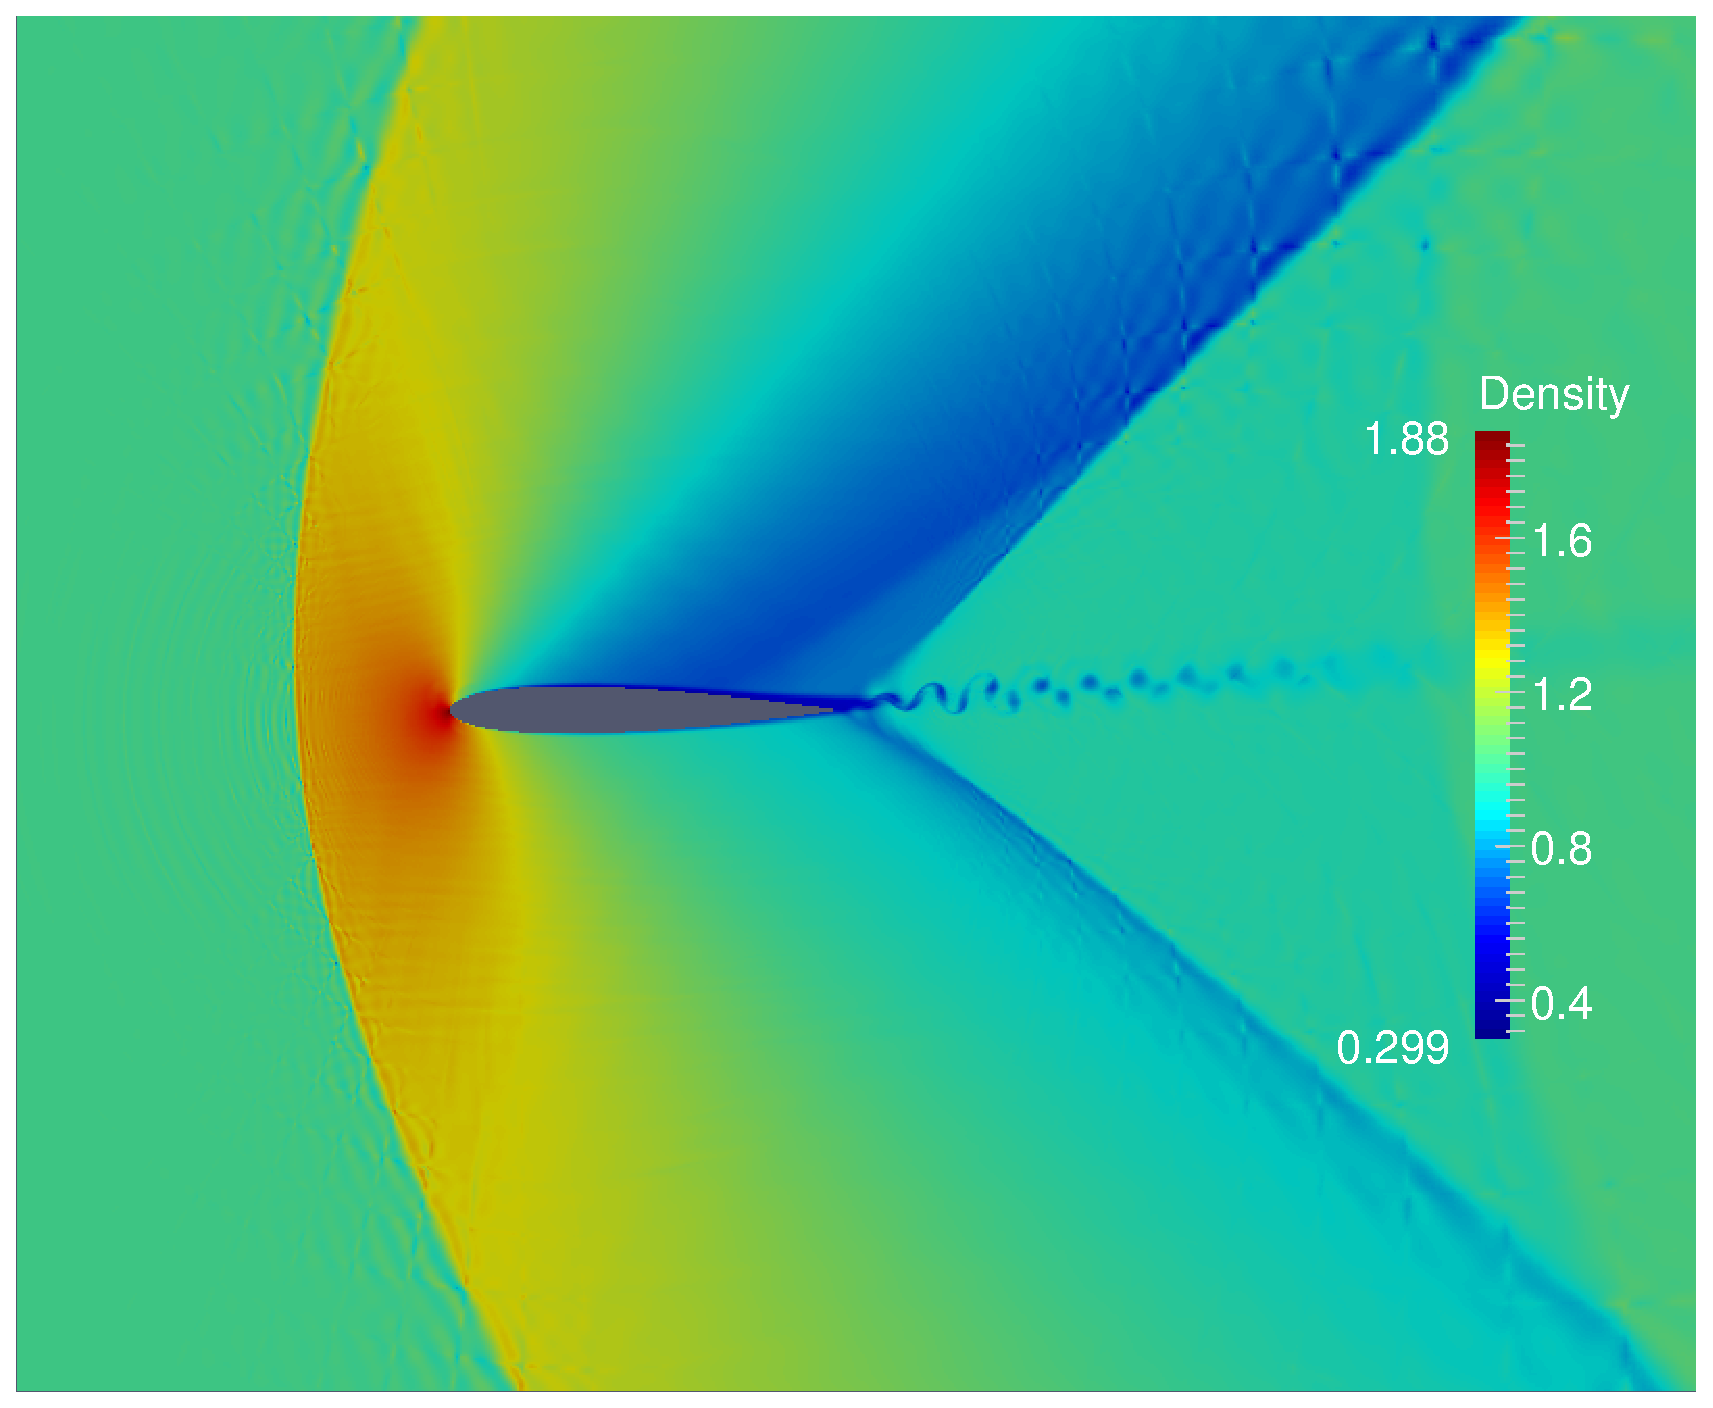
\includegraphics[width=.85\linewidth]{\aiaafigs /density-t1050010-jet.eps}
  \captionof{figure}{density contours for viscous flow at \gls{ma} = 1.2 over a NACA 0012 airfoil at 5$^{\circ}$ \gls{aoa} with polynomial order 6}
  \label{fig:visM1pt2-density}
\end{minipage}%
\begin{minipage}[t]{.5\textwidth}
  \centering
  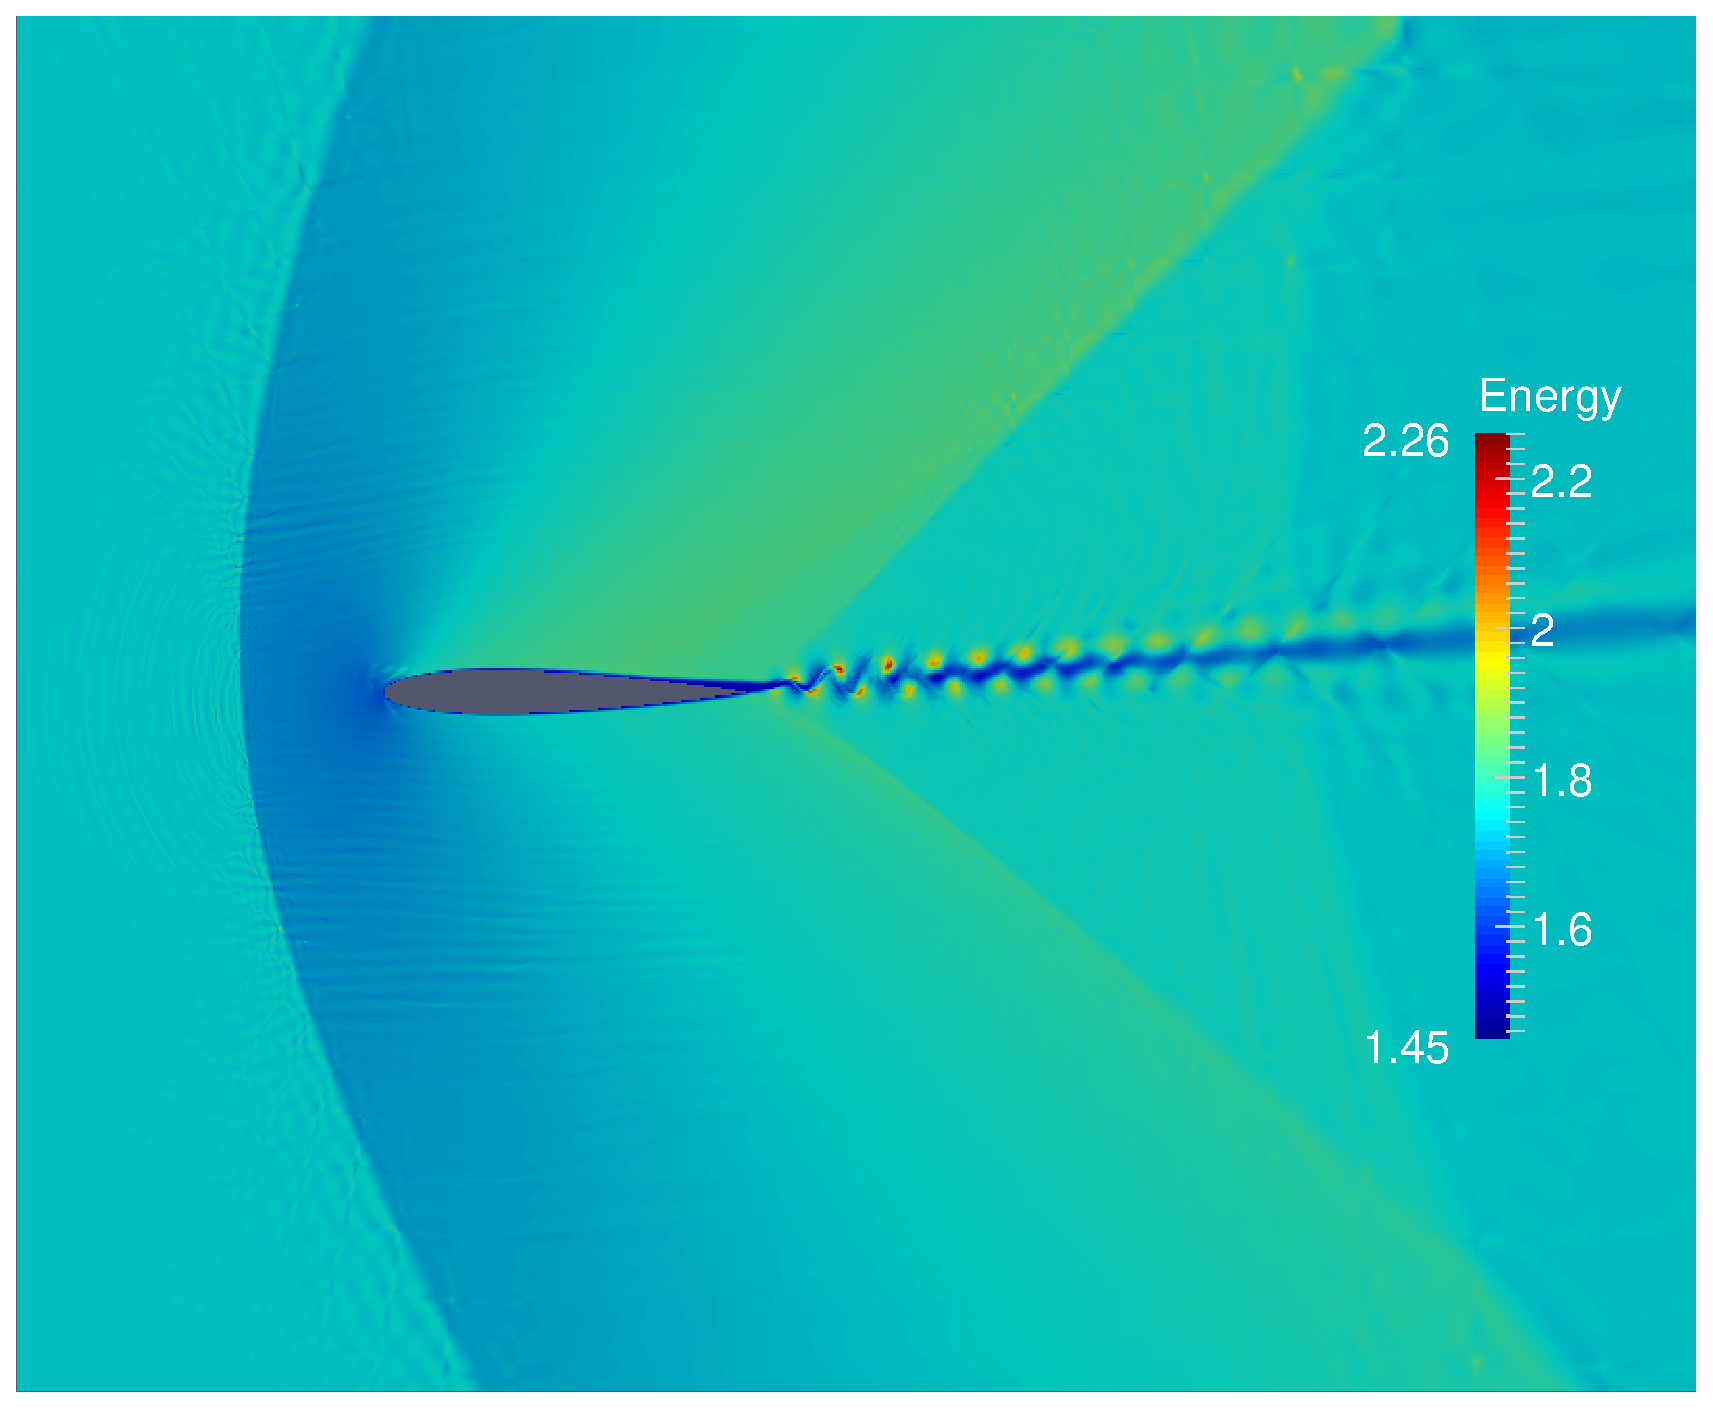
\includegraphics[width=.85\linewidth]{\aiaafigs /energy-t1050010-jet.eps}
  \captionof{figure}{Energy contours}
  \label{fig:visM1pt2-energy}
\end{minipage}
\end{figure} 

\begin{figure}[h] \tt
\centering
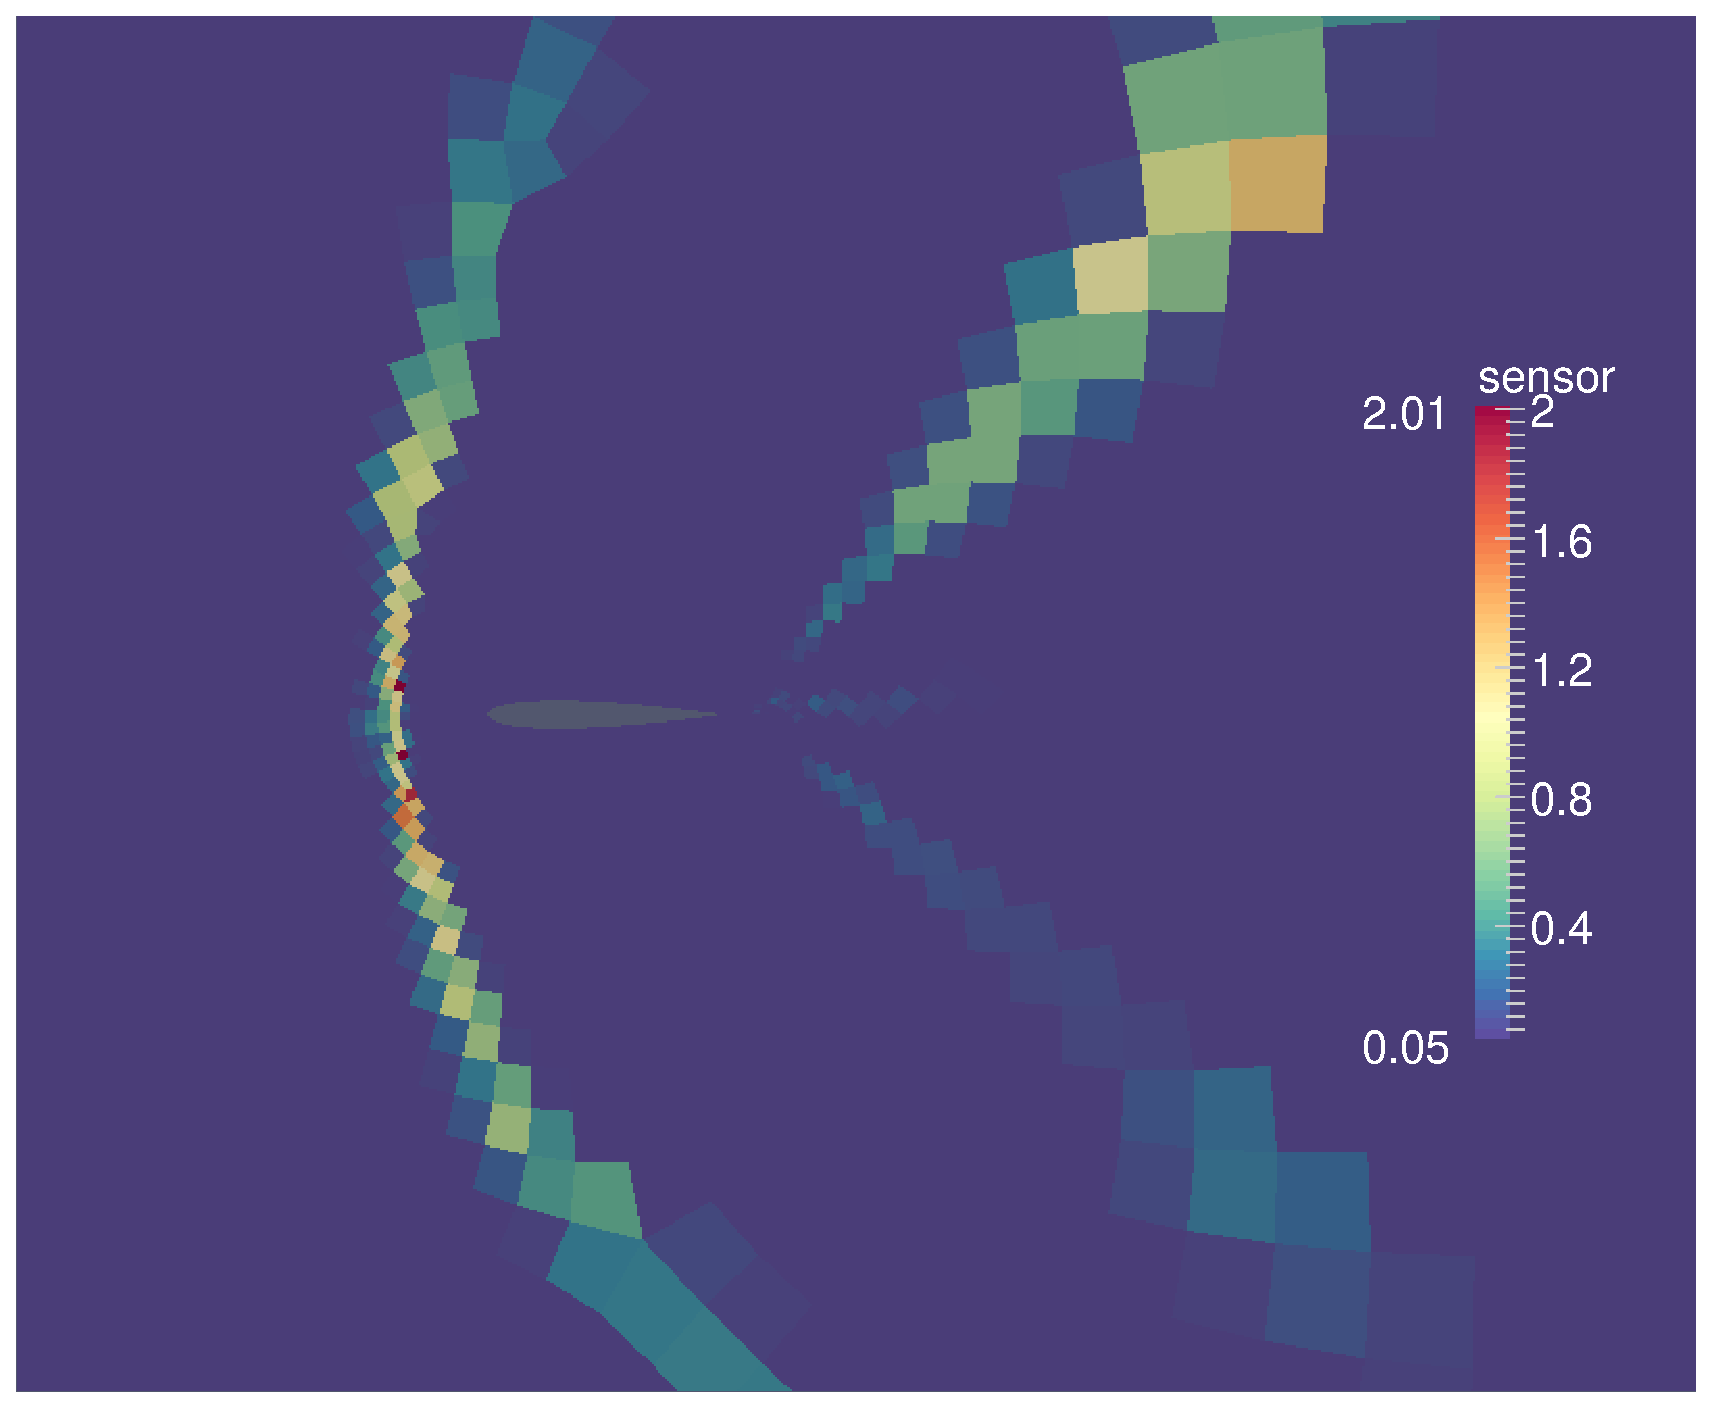
\includegraphics[width = 0.5\textwidth]{\aiaafigs /sensor-t1050010-spectral.eps}
\caption{Figure shows the elemental shock ``sensor'' for the \gls{ma} = 1.2 viscous case shown in figure ~\ref{fig:visM1pt2-density}. The shock sensor is just the maximum value of the enhanced kernel in each element}
\label{fig:sensor}
\end{figure}

\begin{figure}[h] \tt
\centering
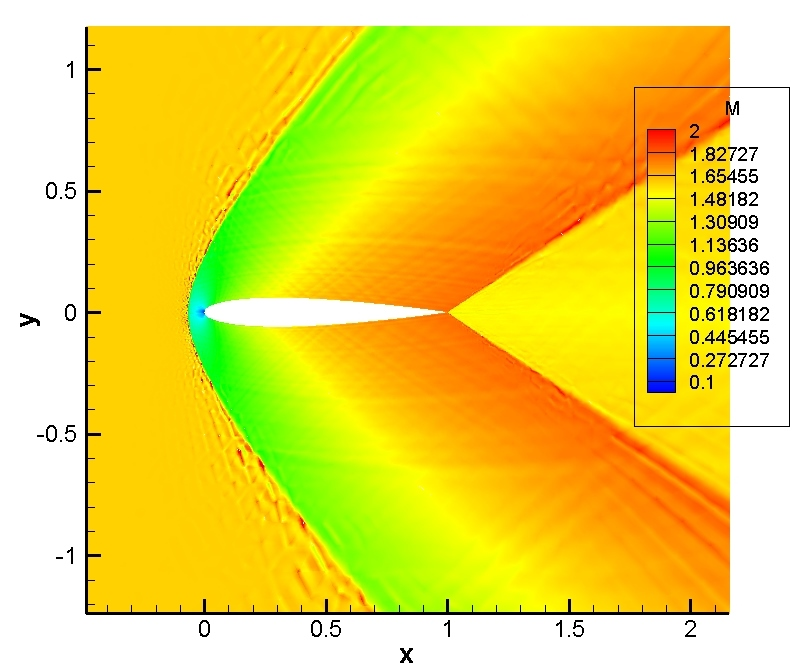
\includegraphics[width = 0.5\textwidth]{\aiaafigs /M1pt6order3-inv-720ktime-mach.jpg} \\
\caption{\gls{ma} contours for inviscid flow over NACA0012 at \gls{ma} = 1.6 and \gls{aoa} = $0^{\circ} $ on a triangle-mesh using Persson and Peraire's method and using artificial viscosity}
\label{fig:inv_mach}
\end{figure}

\begin{figure}
\centering
\begin{minipage}[t]{.55\textwidth}
  \centering
  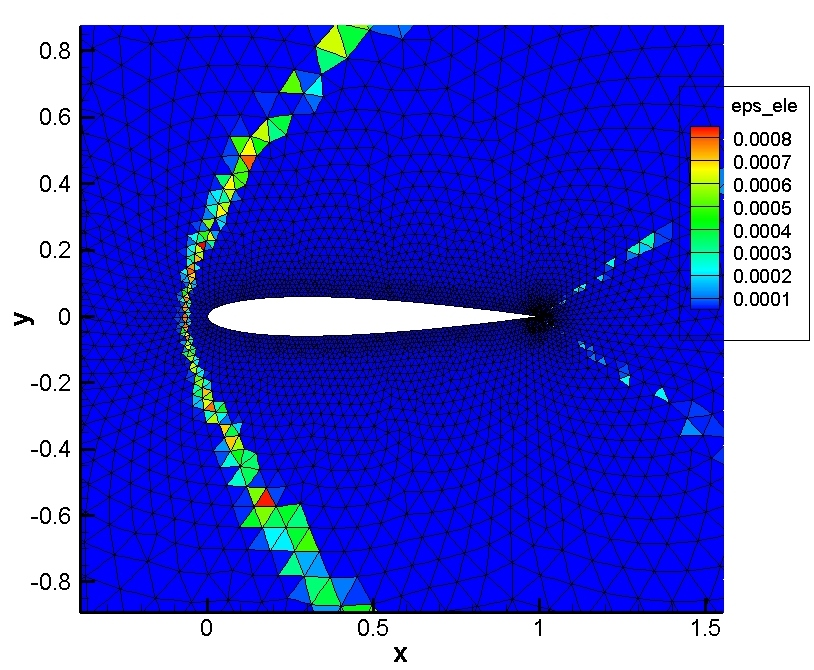
\includegraphics[width=.85\linewidth]{\aiaafigs /M1pt6-inv-av-ele-mesh}
  \caption{Element-wise \gls{av} coefficients for the inviscid \gls{ma}= 1.6 case}
  \label{fig:AV-ele}
\end{minipage}%
\begin{minipage}[t]{.55\textwidth}
  \centering
  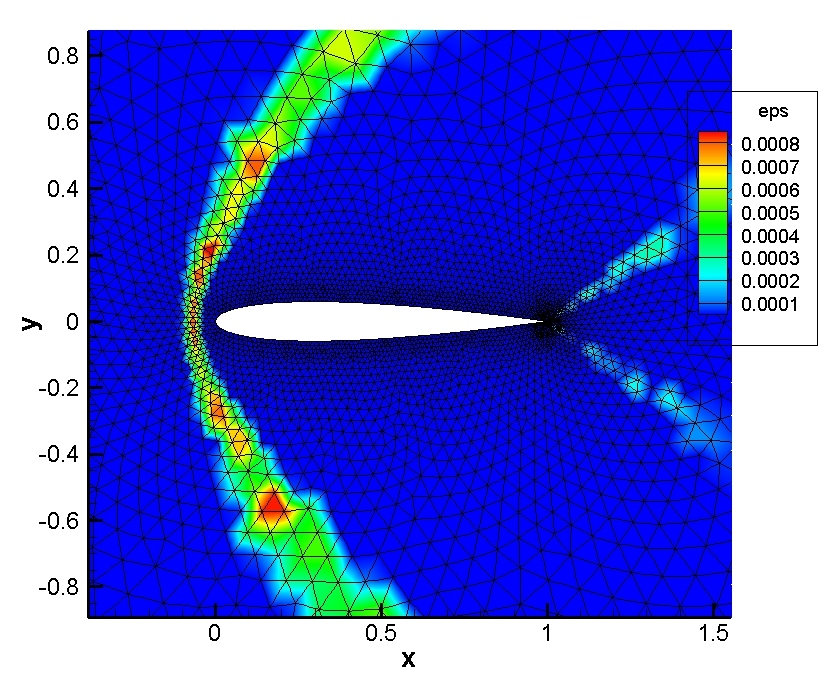
\includegraphics[width=.85\linewidth]{\aiaafigs /M1pt6-inv-av-mesh}
  \caption{\gls{av} coefficients with continuity enforcement}
  \label{fig:AV-cont}
\end{minipage}
\end{figure} 

\subsection{\gls{sa} Turbulence Model and Negative $\tilde\nu$ Modification}

The one equation \gls{sa} turbulence model is one of the more commonly used turbulence models used to solve attached and moderately separated aerodynamic flows~\cite{spalart1992one}. The added equation directly solves for turbulent eddy viscosity via advection, diffusion, production and dissipation. A modified form of the equation can be written as \cite{burgess2012robust,oliver2008high,moro2011navier}:
\begin{equation}
\begin{split}
	\frac{\partial}{\partial t}(\rho\tilde\nu) + \nabla\cdot(\rho\tilde\nu\boldsymbol{u}) = c_{b_1}\tilde S \rho\nu\psi &+ \frac{1}{\sigma}\left[\nabla\cdot((\mu + \mu\psi)\nabla\tilde\nu) + c_{b_2}\rho\nabla\tilde\nu\cdot\nabla\tilde\nu\right] \\&- c_{w_1}\rho f_w \left(\frac{\nu\psi}{d}\right)^2
\end{split}
\end{equation}

where $\tilde\nu$ is a modified version of the kinematic eddy viscosity and $\nu$ is the kinematic viscosity. The other variables are defined as:

\begin{align}
	 \mu_t =
	  \begin{cases}
	   \rho\tilde\nu f_{v_1} & \text{if } \tilde\nu \ge 0 \\
	   0       & \text{if } \tilde\nu < 0
	  \end{cases}
	  \quad \mbox{where} \quad f_{v_1} = \frac{\left(\frac{\rho\tilde\nu}{\mu}\right)^3}{\left(\frac{\rho\tilde\nu}{\mu}\right)^3 + c_{v_1}^3}
\end{align}

\begin{align}
	\tilde S &=
	\begin{cases}
	   S + \bar S & \text{if } \bar S \ge -c_{v_2}S \\
	   S + \frac{S(c_{v_2}^2 S + c_{v_3}\bar S)}{(c_{v_3} - 2c_{v_2})S - \bar S} & \text{if } \bar S \le -c_{v_2}S
	\end{cases}
\end{align}
\begin{align}
	S &= \sqrt{\boldsymbol{\omega}\cdot\boldsymbol{\omega}}
	\qquad \bar S = \frac{(\nu\psi)^2 f_{v_2}}{\kappa^2 d^2} \\
	f_{v_2} &= 1 - \frac{\psi}{1 + \psi f_{v_1}}
\end{align}

\begin{align}
	f_w &= g\left[\frac{1 + c_{w_3}^6}{g^6 + c_{w_3}^6}\right]^{1/6} 
	\qquad g = r + c_{w_2}(r^6 - r) 
	\qquad r = \frac{\nu\psi}{\tilde S \kappa^2 d^2}
\end{align}

where S is the magnitude of vorticity, d is the closest distance to a wall, $c_{b1} = 0.1355$, $\sigma = \frac{2}{3}$, $c_{b2} = 0.622$, $K = 0.41$, $\text{Pr}_t = 0.9$, $c_{v1} = 7.1$, $c_{v2} = 0.7$, $c_{v3} = 0.9$, $c_{w1} = \frac{c_{b1}}{K^2} + \frac{(1+c_{b2})}{\sigma}$, $c_{w2} = 0.3$, $c_{w3} = 2$.\\

The diffusion term, $\nabla\cdot(\rho\tilde\nu\boldsymbol{u})$, may become discontinuous in the first derivative leading to oscillations in high-order polynomials. This can lead to large negative values of the modified eddy viscosity term, $\tilde\nu$, significant enough to cause an unbounded solution. To prevent this, the following modification is introduced \cite{moro2011navier}.
\begin{align}
	\psi &=
	\begin{cases}
	   0.05log(1.0 + e^{(20.0\chi)}) & \text{if } \chi \le 10.0, \\
	   \chi & \text{if } \chi > 10.0,
	\end{cases} \\
	\chi &= \frac{\tilde\nu}{\nu}
\end{align}

\subsection{Large Eddy Simulation}\label{lesmodels}

In order to resolve all the scales of motion in a high \gls{re} number turbulent flow, the computational mesh would have to be exceedingly fine.
A practical solution is to employ the \gls{les} formulation, which only resolves the larger scales of motion and thus allows for the use of coarser meshes.

The effect of the unresolved or \gls{sgs} dynamics on the solution is accounted for by an \gls{sgs} model for the subgrid-scale stress $\tau_{ij}$, which is added to the viscous stress tensor $\sigma_{ij}$ given by (\ref{sigma}):

\begin{eqnarray}\label{tausgs}
\sigma_{ij} &&= 2 \mu S^d_{ij} + \tau_{ij},\\
S^d_{ij} &&= \frac 1 2 \l( \frac{\partial u_i}{\partial x_j} + \frac{\partial u_j}{\partial x_i} - \frac{2}{3} \delta_{ij}\frac{\partial u_k}{\partial x_k} \r).
\end{eqnarray}

The standard Smagorinsky model~\cite{smagorinsky1963} is available in \gls{hf}:
\begin{eqnarray}\label{smag}
\tau_{ij} &&= 2 \mu_t S^d_{ij}, \\
\mu_t &&= \rho C_S^2 \bigtriangleup^2 | S^d |,\\
| S^d | &&= \sqrt{2 S^d_{ij} S^d_{ij}},
\end{eqnarray}
where $\mu_t$ is the eddy viscosity, $C_S = 0.1$ is the Smagorinsky coefficient and $\bigtriangleup$ is the filter width. In \gls{hf} the filter width is given by (in 3D):
\begin{equation}
\bigtriangleup = \alpha (\text{vol})^{1/3},
\end{equation}
where $\alpha \geq 1$ is a user-defined scaling factor and vol is the element volume.

\gls{hf} also includes the \gls{wale} model~\cite{nicoud1999} and the Similarity model~\cite{bardina1980}.
The Similarity model incorporates a low-pass filtering operator, for which several choices are available in \gls{hf}: a discrete Gaussian filter\cite{lodato2012b}, a high-order commuting Vasilyev-type filter\cite{vasilyev1998,vasilyev2001} and a modal Vandermonde-type filter\cite{blackburn2003}.

The modal filter can be used on unstructured tetrahedral meshes. For details of these operators, see Lodato, Castonguay and Jameson~\cite{lodato2012b} and Bull and Jameson~\cite{bull2014a}. One can combine the similarity model with the Smagorinsky or \gls{wale} model to form a mixed \gls{sgs} model. The \gls{wsm} model, first proposed by Lodato et al.~\cite{lodato2009}, was used in simulations of the flow over a square cylinder (see Section~\ref{sqcyl}).

\subsection{Computing Architecture and Scalability}

The \gls{hf} code has been designed to work on multi-CPU as well as multi-CPU-\gls{gpu} platforms. The \gls{fr} method in its current form with explicit time-stepping has a great potential for parallelization. Since the solution points are not explicitly shared between elements, most of the computations are element-local enabling an efficient use of shared memory on \gls{gpu}s. Also, several computations are independent for each solution point and the highly parallelizable nature of \gls{gpu}s becomes very useful. A detailed description of the parallelization of the \gls{fr} method, along with scalability and performance analysis has been performed in~\cite{castonguay2011}.